
\begin{frame}[ctb!]
  \frametitle{Demonstration Case : Code Development}
  \begin{figure}[htbp!]
    \begin{center}
      \includegraphics[height=.5\textheight]{cyder/images/componentLoading.eps}
      \caption{A number of base cases were run to investigate the performance of 
      the nuclide transport models.}
    \end{center}
  \end{figure}
\end{frame}


\begin{frame}
  \frametitle{Output Tables}
  Currently, there are three GenericRepository related output tables. This 
  number will increase as more thermal and  nuclide transport data becomes 
  necessary.

  \begin{itemize}
  \item \textbf{gen\_repo\_params} : This table keeps data from the query engine 
    that parameterized the generic repository, for reproducibility.
  \item \textbf{gen\_repo\_components} : This table keeps data that 
    parameterized each component, both from the query engine and from the 
    GenericRepository procedures that position and arrange these components. 
  \item \textbf{gen\_repo\_contaminants} : This table keeps track of the 
    isotopic composition of the contaminants in each component as they move 
    radially outward. 
\end{itemize}
\end{frame}


\begin{frame}
  The NuclideModel in a Component can be interchangeably represented by any of 
  the four nuclide transport models. 
    \begin{itemize}
      \item Degradation Rate Based Failure Model
      \item Mixed Cell with Degradation, Sorption, Solubility Limitation
      \item Lumped Parameter Model
      \item 1D Advection Dispersion Solution
    \end{itemize}
\end{frame}

\begin{frame}
  \frametitle{Degradation Rate Base Cases}
  A DegRateNuclide model is defined solely by its degradation rate and the 
  advective velocity of the system. 

  Cases were run with all components being represented by the DegRateNuclide 
  model.  
\end{frame}


\begin{frame}
  \frametitle{Degradation Rate Base Case I}
  Base Case I : If the degradation rate of the waste form is 0, then no nuclides should be 
  transported out of it, irrespective of the degradation rates of other 
  barriers. 

  \begin{figure}[htbp!]
    \begin{center}
      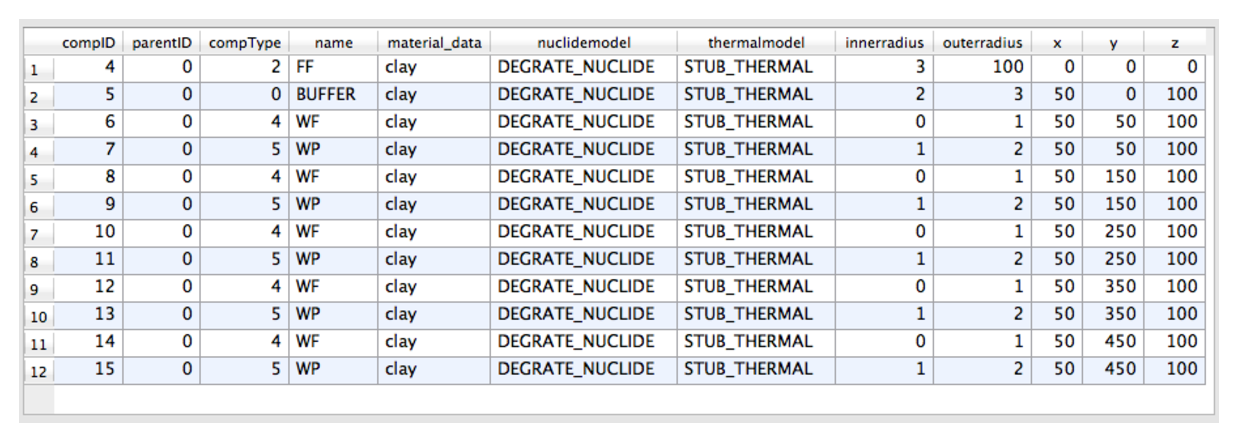
\includegraphics[width=\textwidth]{cyder/images/stub_0deg_comp_table.eps}
    \end{center}
  \end{figure}
\end{frame}

\begin{frame}
  \frametitle{Degradation Rate Base Case I}
  Base Case I : If the degradation rate of the waste form is 0, then no nuclides should be 
  transported out of it, irrespective of the degradation rates of other 
  barriers. 

  \begin{figure}[htbp!]
    \begin{center}
      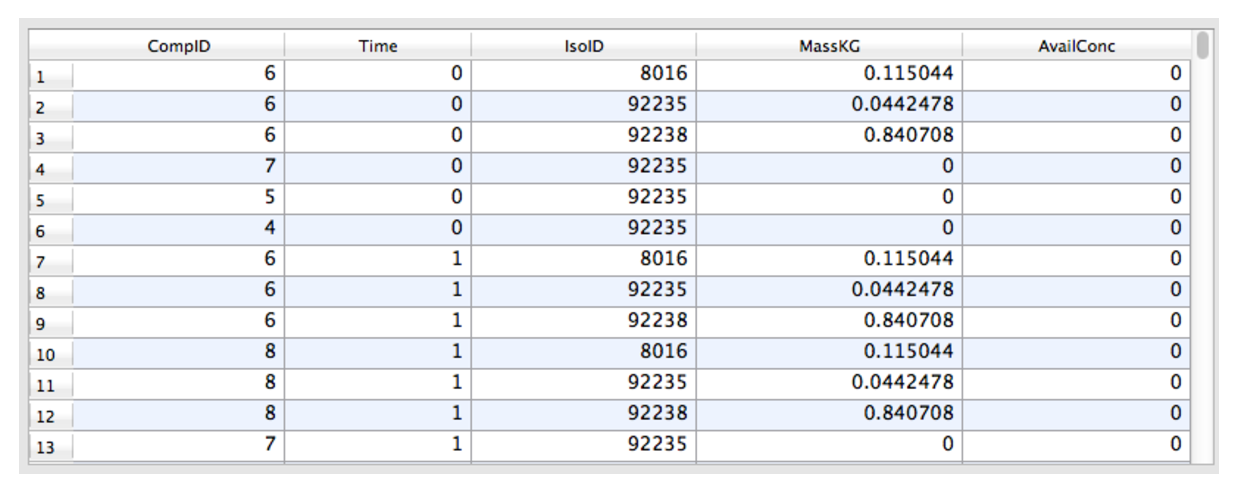
\includegraphics[width=\textwidth]{cyder/images/stub_0deg_cont_table.eps}
      \caption{A number of base cases were run to investigate the performance of 
      the nuclide transport models.}
    \end{center}
  \end{figure}
\end{frame}

\begin{frame}
  \frametitle{Degradation Rate Base Case I}
  Base Case I : If the degradation rate of the waste form is 0, then no nuclides should be 
  transported out of it, irrespective of the degradation rates of other 
  barriers. 

  \begin{figure}[htbp!]
    \begin{center}
      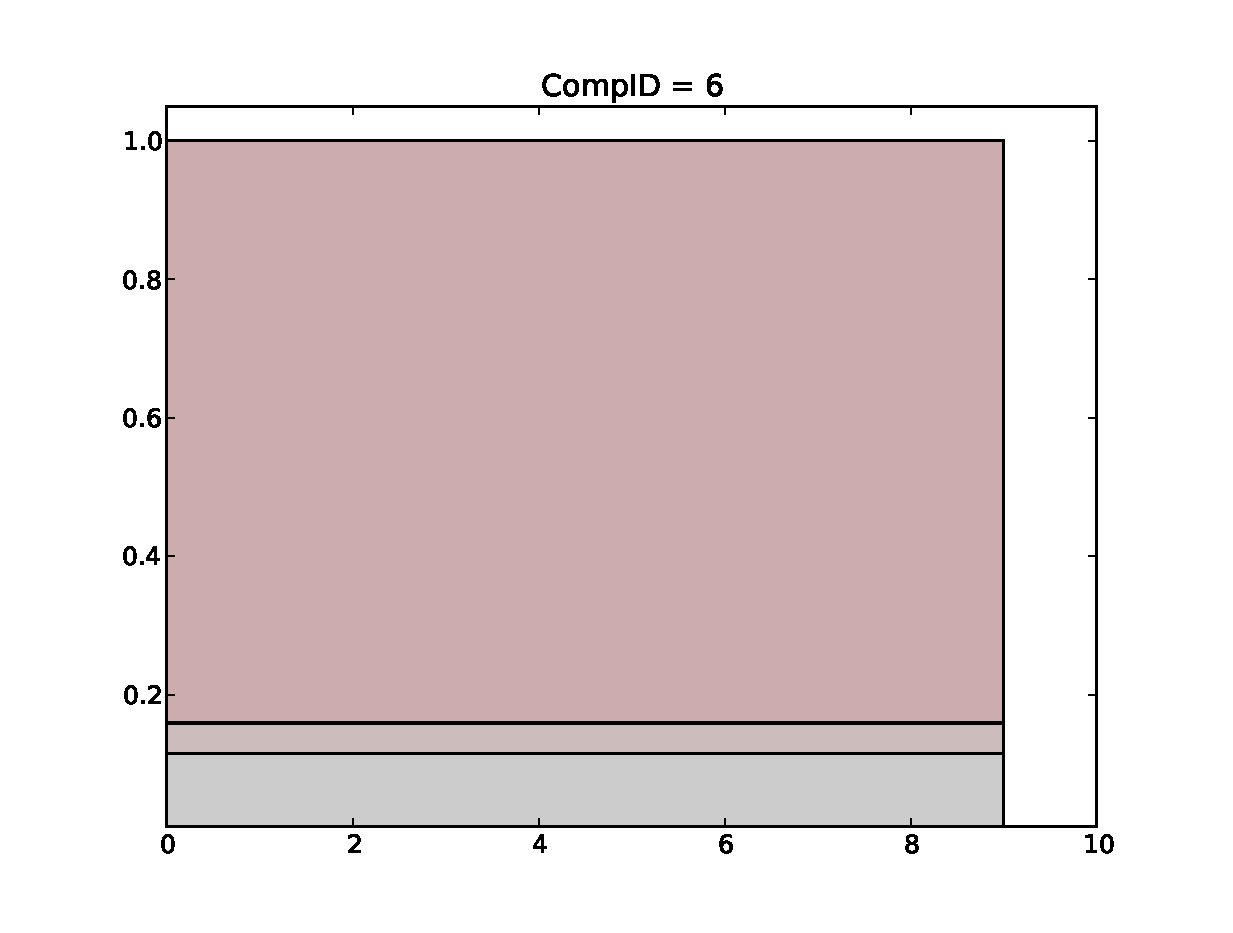
\includegraphics[width=.5\textwidth]{cyder/images/0deg_comp6.eps}
      \includegraphics[width=.5\textwidth]{cyder/images/0deg_comp7.eps}
    \end{center}
  \end{figure}
\end{frame}

\begin{frame}
  \frametitle{Degradation Rate Base Case I}
  Base Case I : If the degradation rate of the waste form is 0, then no nuclides should be 
  transported out of it, irrespective of the degradation rates of other 
  barriers. 

  \begin{figure}[htbp!]
    \begin{center}
      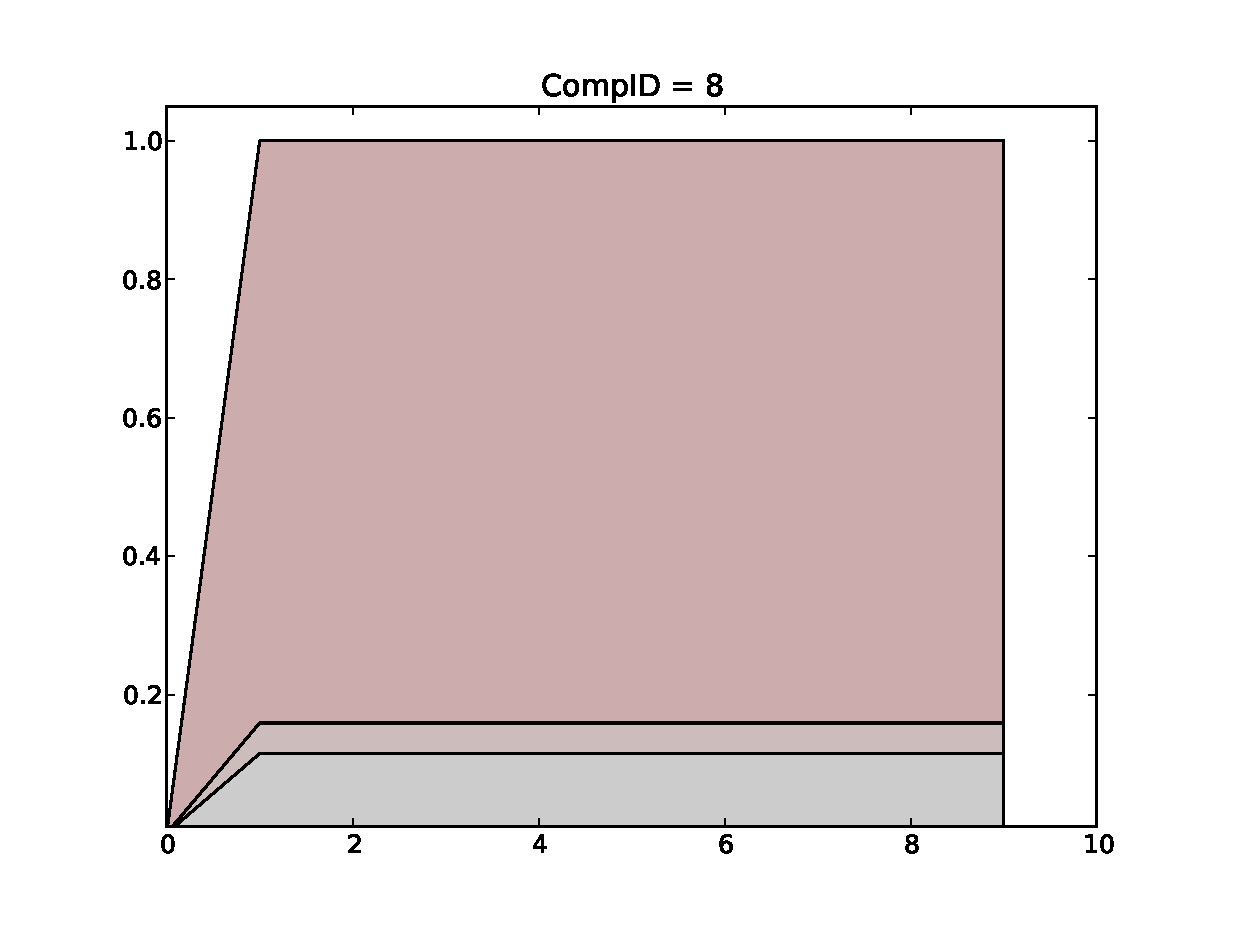
\includegraphics[width=.5\textwidth]{cyder/images/0deg_comp8.eps}
      \includegraphics[width=.5\textwidth]{cyder/images/0deg_comp9.eps}
    \end{center}
  \end{figure}
\end{frame}

\begin{frame}
  \frametitle{Degradation Rate Base Case I}
  Base Case I : If the degradation rate of the waste form is 0, then no nuclides should be 
  transported out of it, irrespective of the degradation rates of other 
  barriers. 

  \begin{figure}[htbp!]
    \begin{center}
      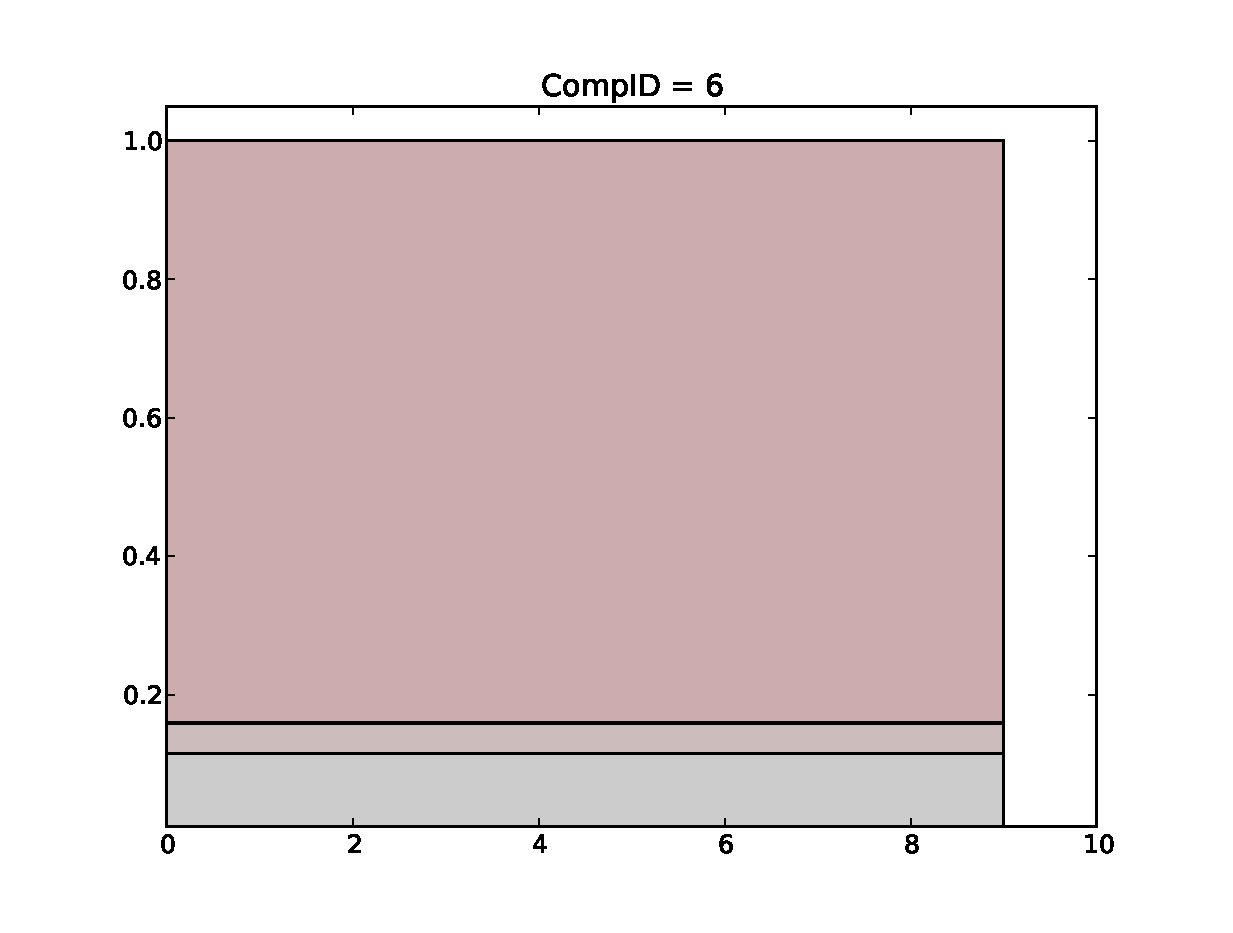
\includegraphics[width=.2\textwidth]{cyder/images/0deg_comp6.eps}
      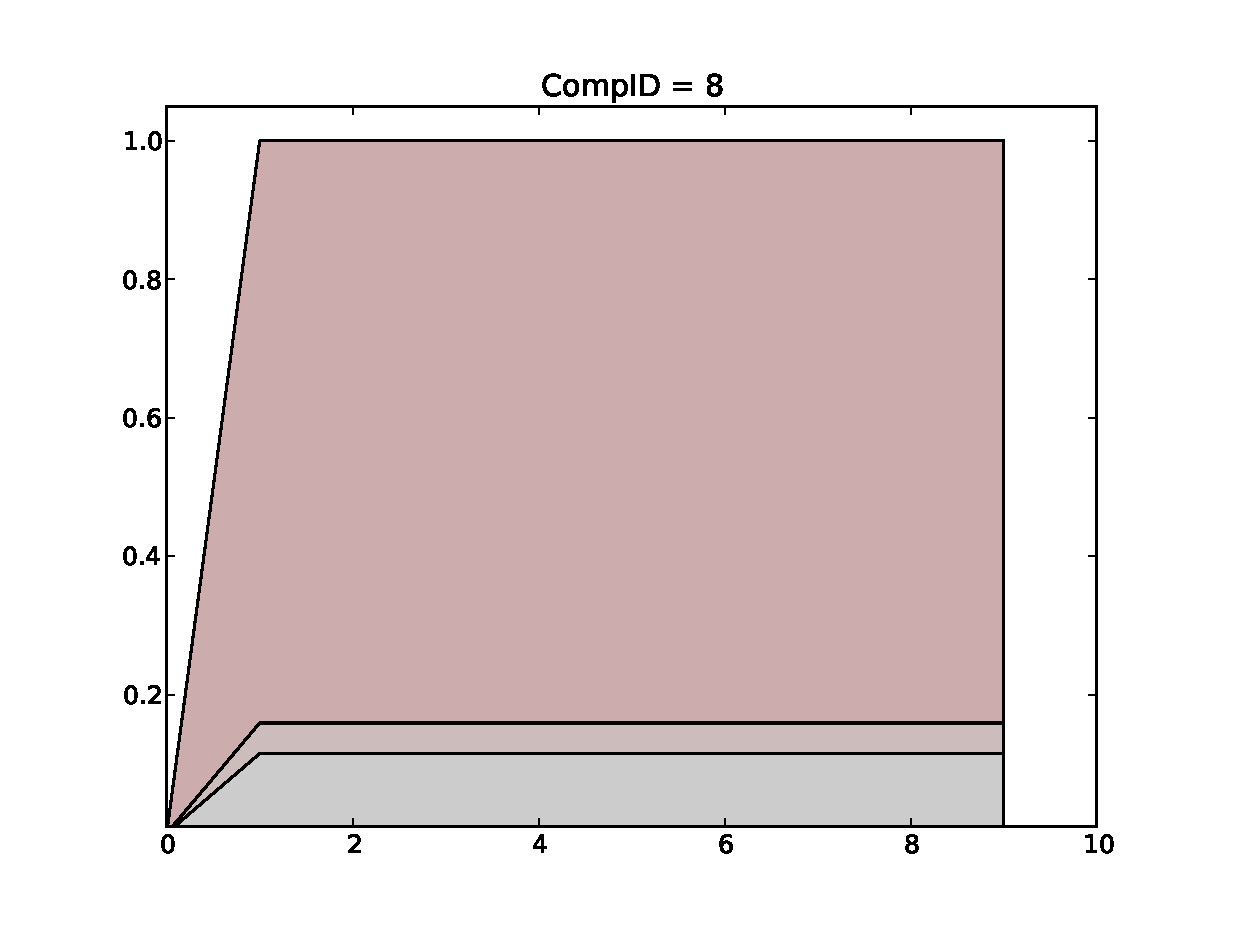
\includegraphics[width=.2\textwidth]{cyder/images/0deg_comp8.eps}
      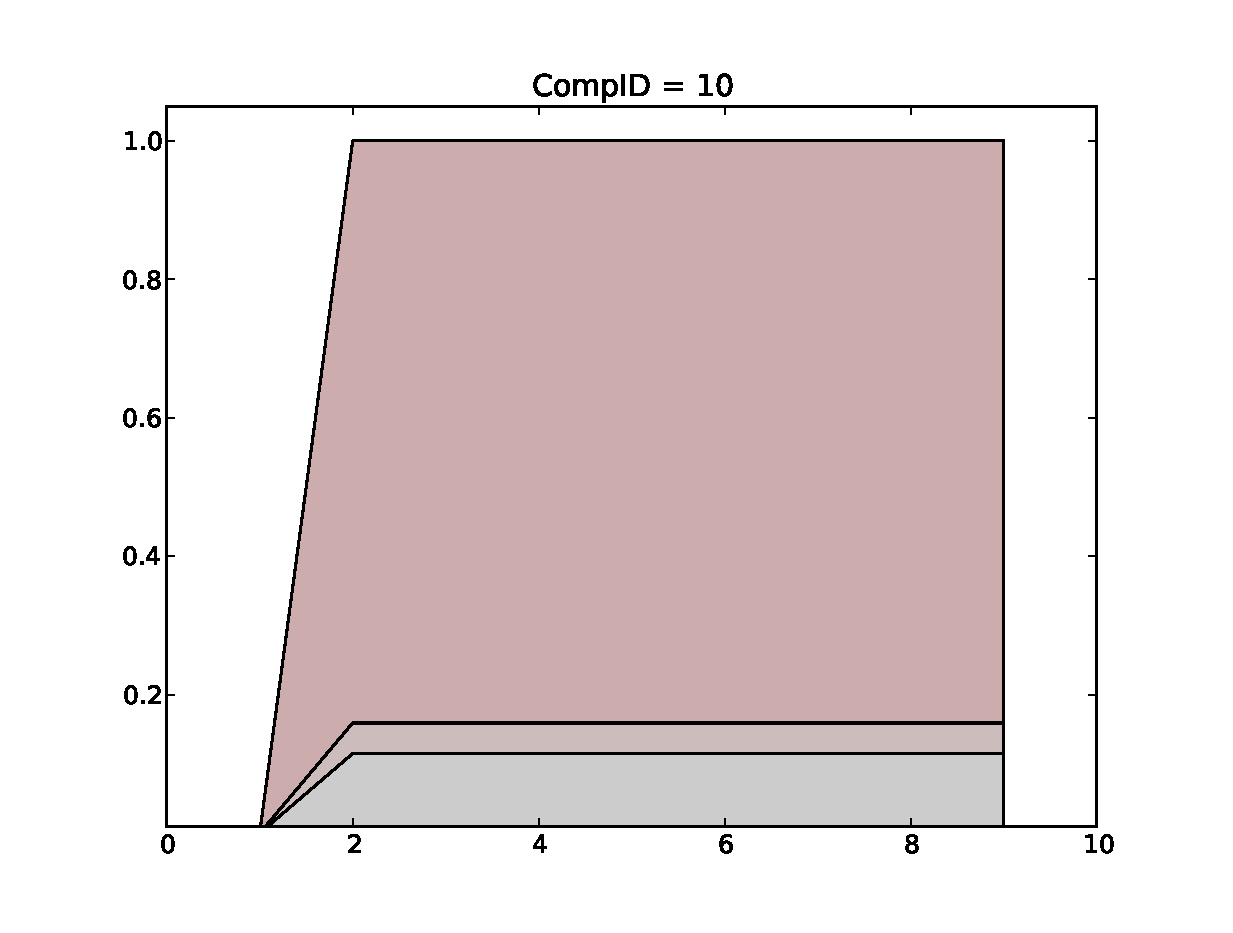
\includegraphics[width=.2\textwidth]{cyder/images/0deg_comp10.eps}
      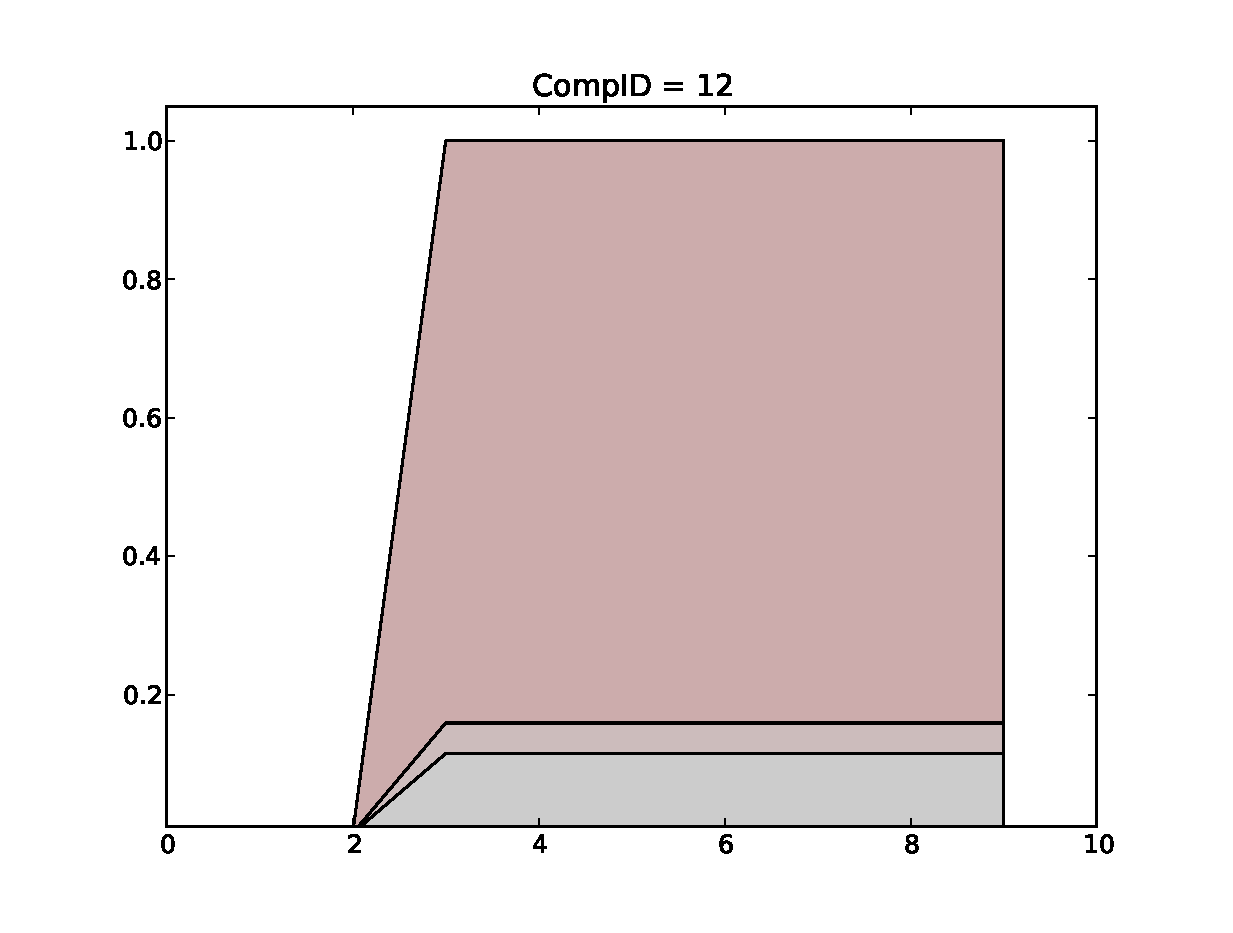
\includegraphics[width=.2\textwidth]{cyder/images/0deg_comp12.eps}
      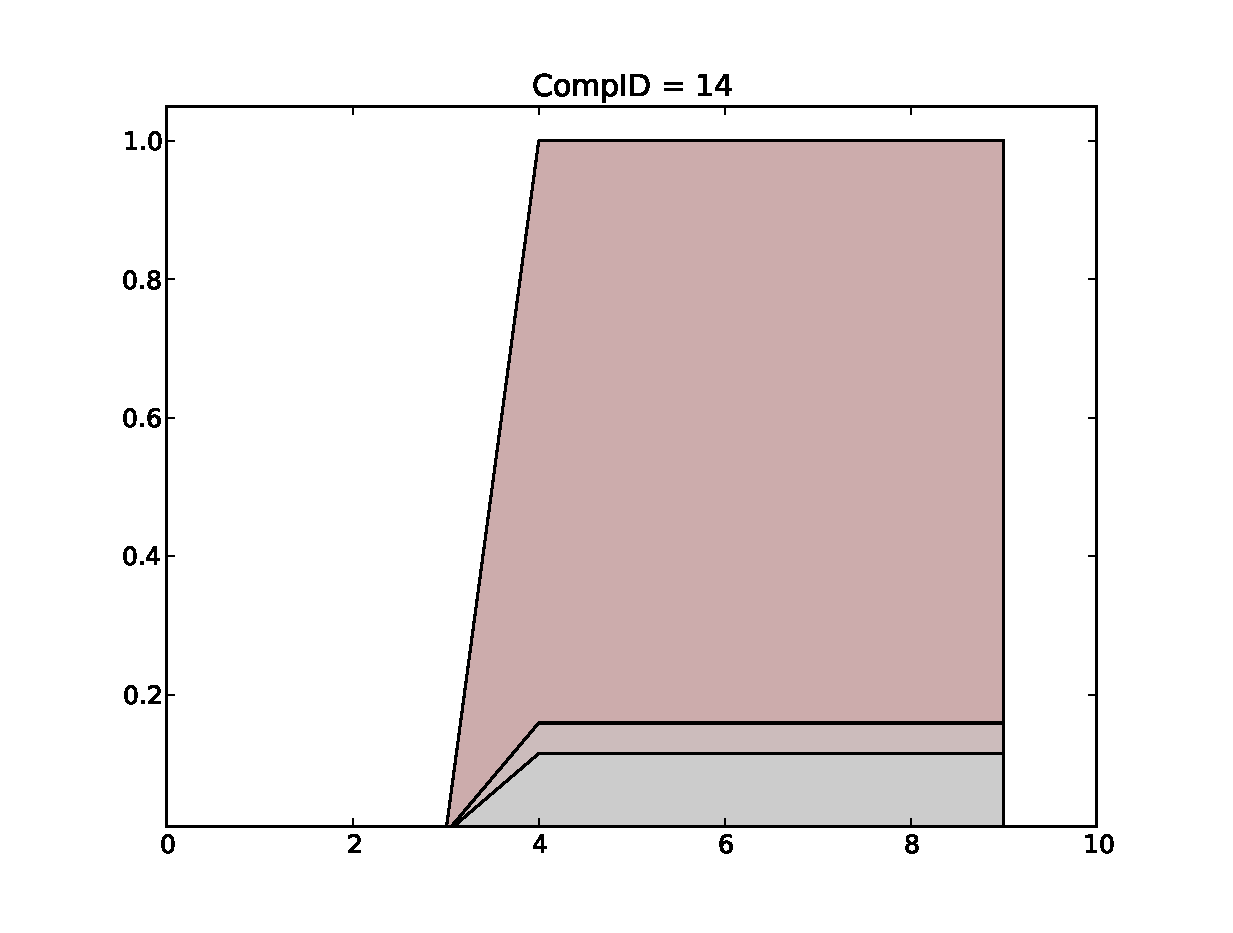
\includegraphics[width=.2\textwidth]{cyder/images/0deg_comp14.eps}
    \end{center}
  \end{figure}
\end{frame}

\begin{frame}
  \frametitle{Degradation Rate Base Case I}
  Base Case I : If the degradation rate of the waste form is 0, then no nuclides should be 
  transported out of it, irrespective of the degradation rates of other 
  barriers. 

  \begin{figure}[htbp!]
    \begin{center}
      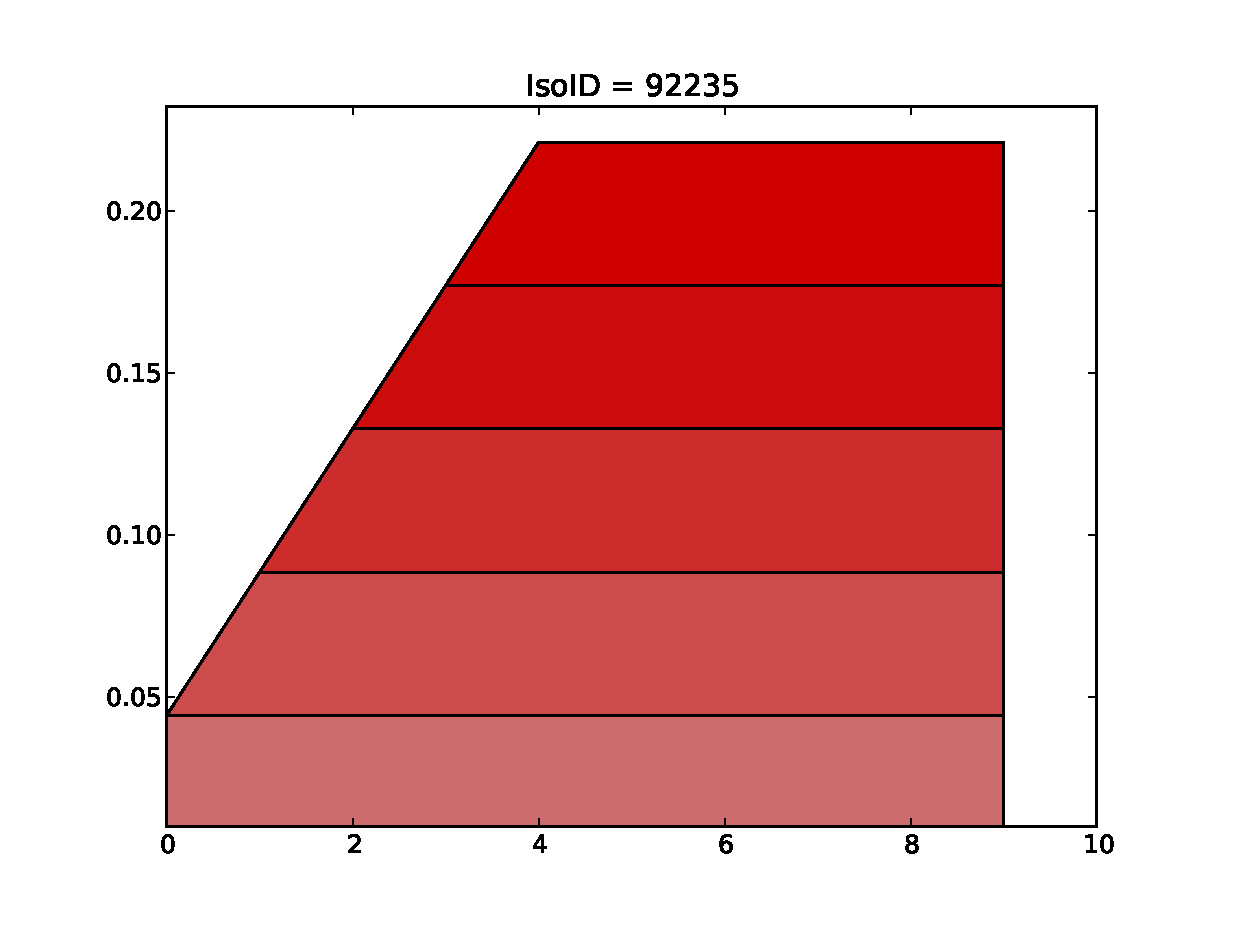
\includegraphics[width=.7\textwidth]{cyder/images/0deg.eps}
    \end{center}
  \end{figure}
\end{frame}


\begin{frame}
  \frametitle{Degradation Rate Base Case II}
  Base Case II : If the degradation rates for all pieces are 10\% per timestep and 
  five waste forms are necessary, the far field should recieve a  small amount
  of material after 4 timesteps.

  \begin{figure}[htbp!]
    \begin{center}
      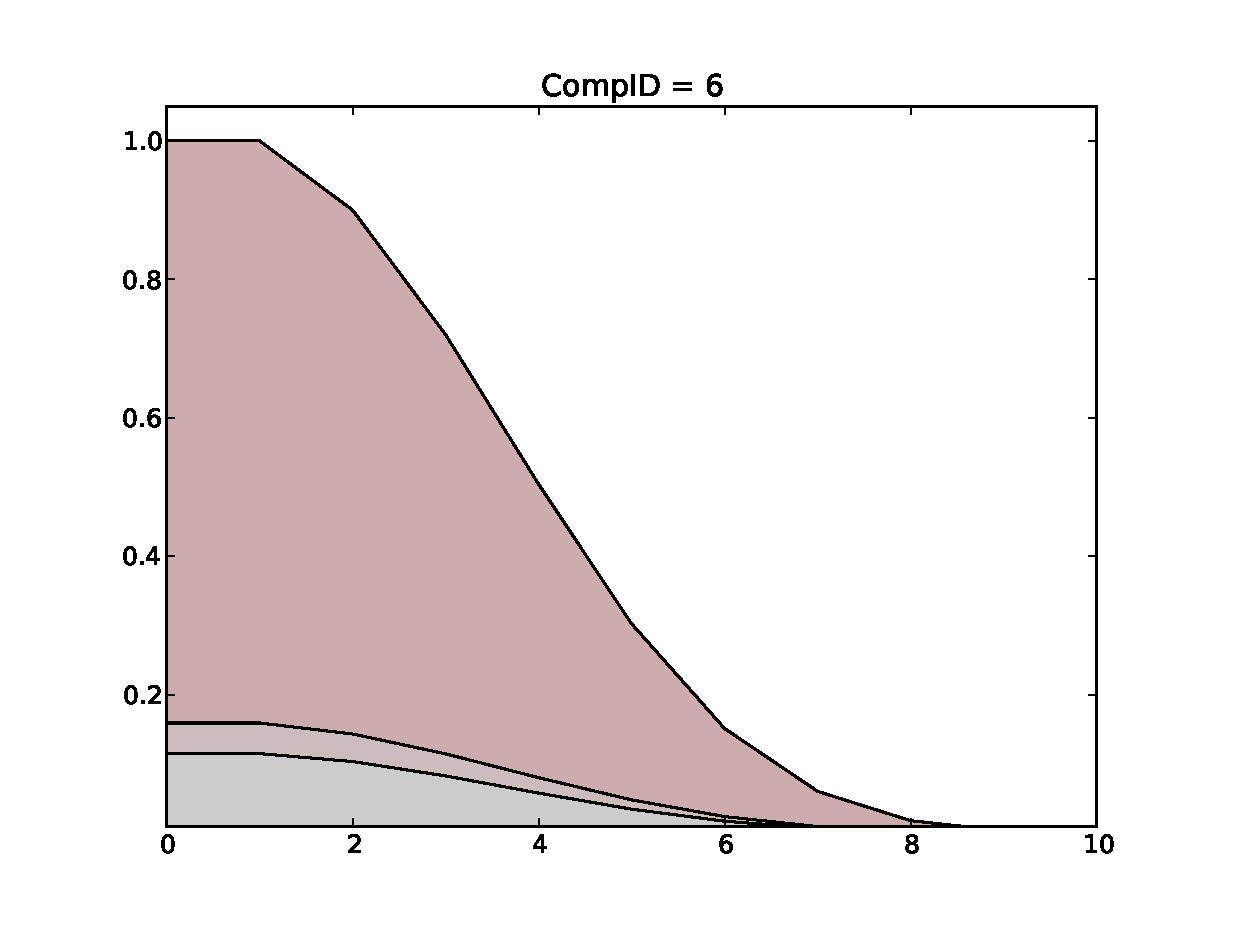
\includegraphics[width=0.5\textwidth]{cyder/images/deg_comp6.eps}
      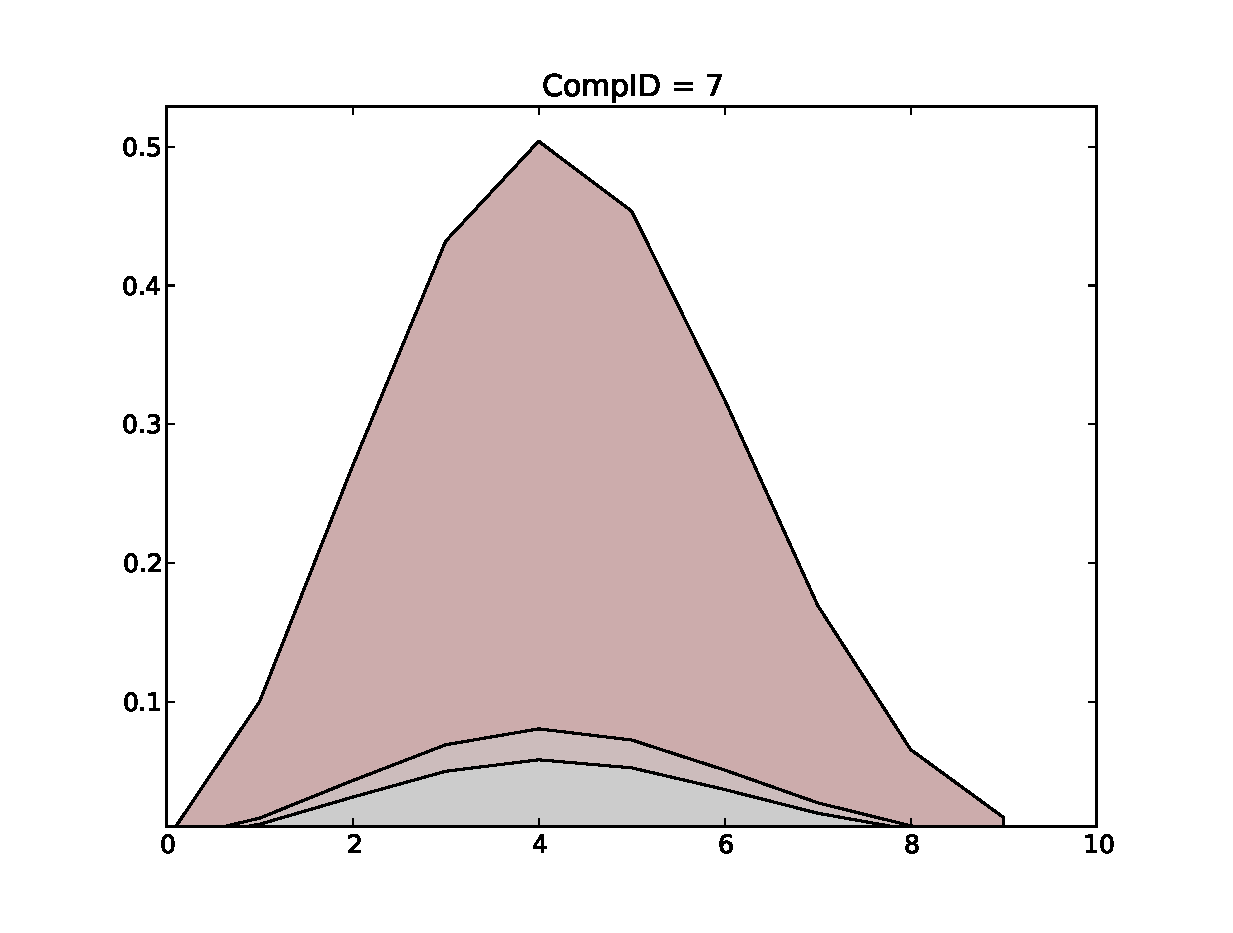
\includegraphics[width=0.5\textwidth]{cyder/images/deg_comp7.eps}
    \end{center}
  \end{figure}
\end{frame}

\begin{frame}
  \frametitle{Degradation Rate Base Case II}
  Base Case II : If the degradation rate of all pieces are 10\% and only one 
  waste form is necessary, the far field should recieve a very small amount
  of material after 4 timesteps.

  \begin{figure}[htbp!]
    \begin{center}
      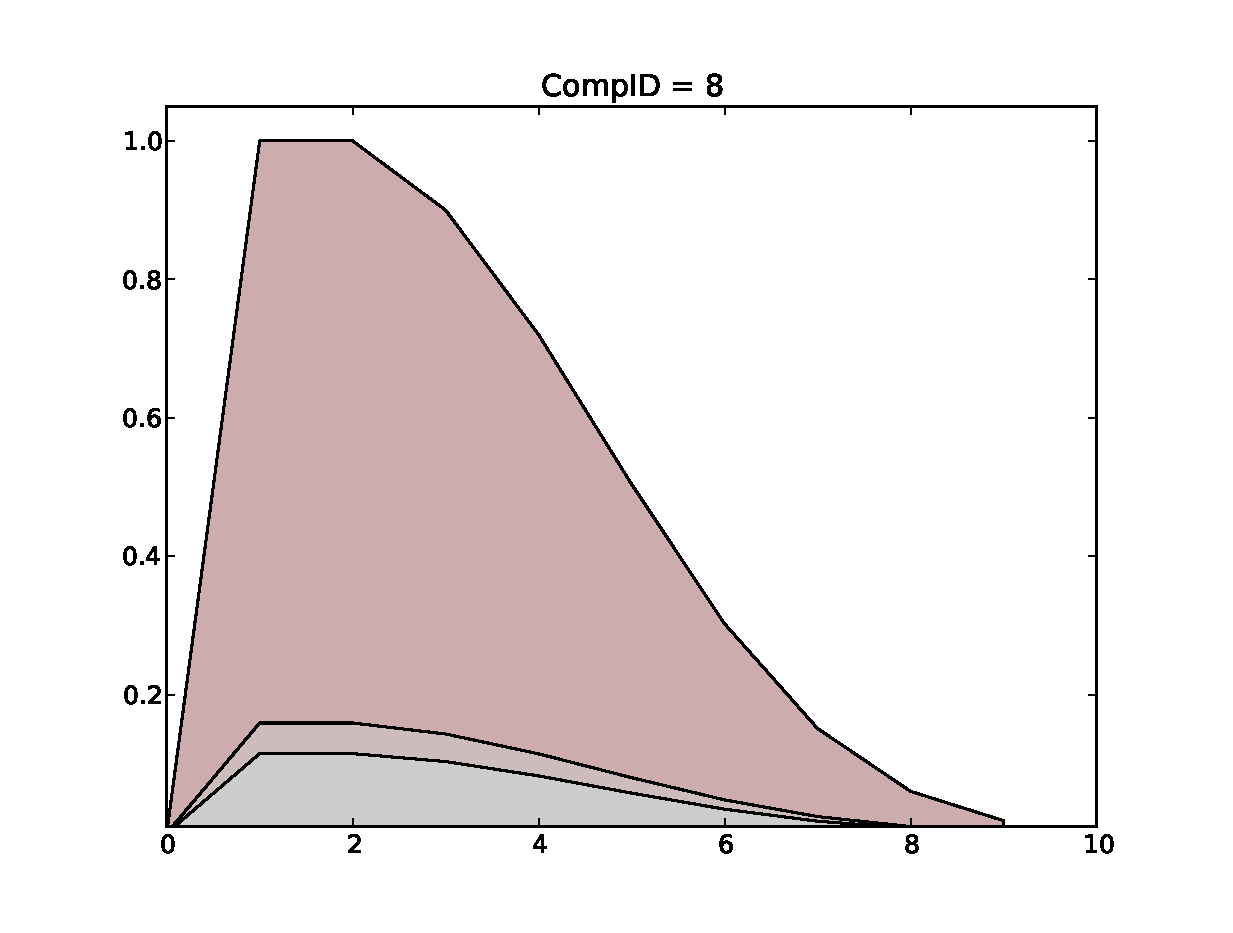
\includegraphics[width=0.5\textwidth]{cyder/images/deg_comp8.eps}
      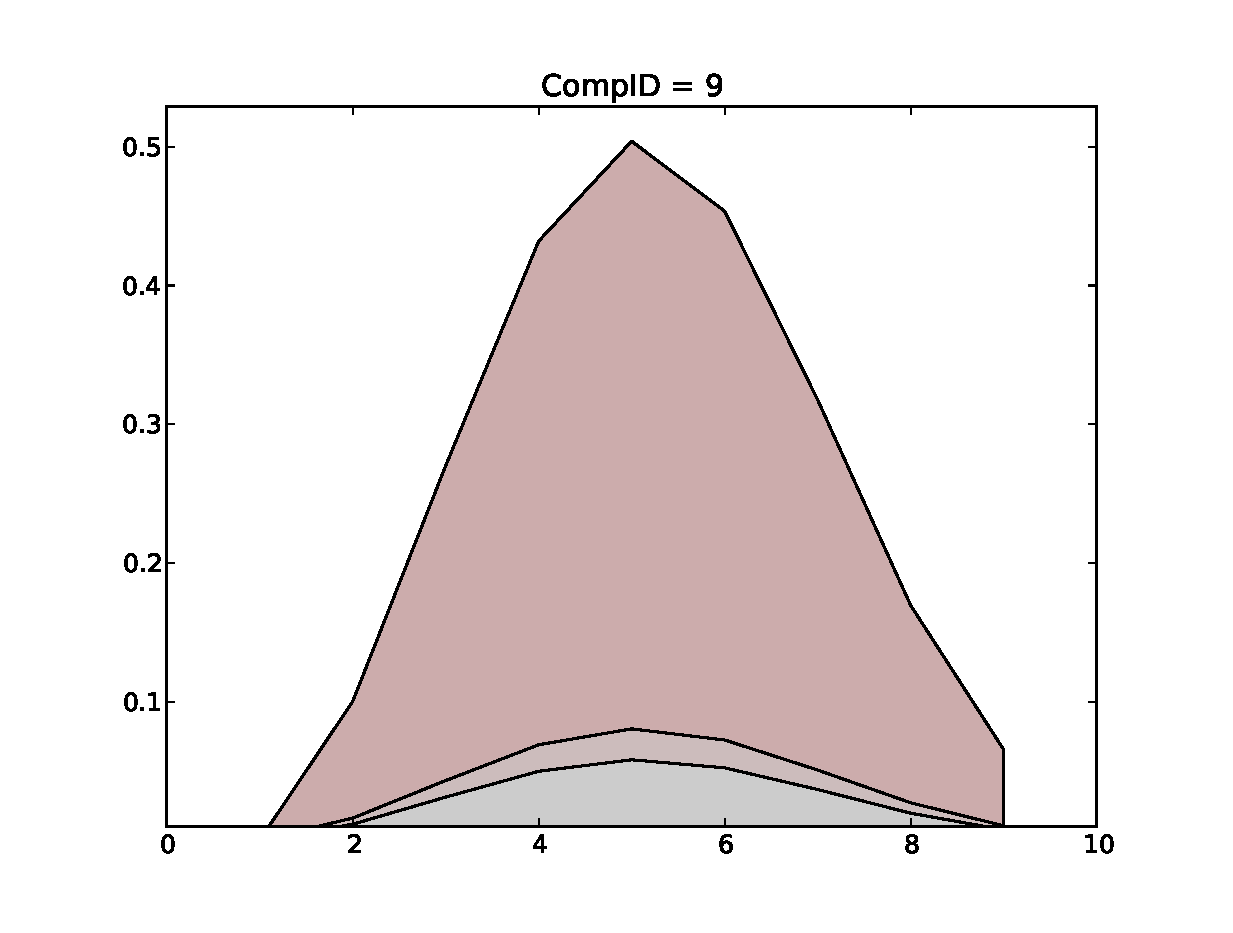
\includegraphics[width=0.5\textwidth]{cyder/images/deg_comp9.eps}
    \end{center}
  \end{figure}
\end{frame}

\begin{frame}
  \frametitle{Degradation Rate Base Case II}
  Base Case II : If the degradation rate of all pieces are 10\% and only one 
  waste form is necessary, the far field should recieve a very small amount
  of material after 4 timesteps.

  \begin{figure}[htbp!]
    \begin{center}
      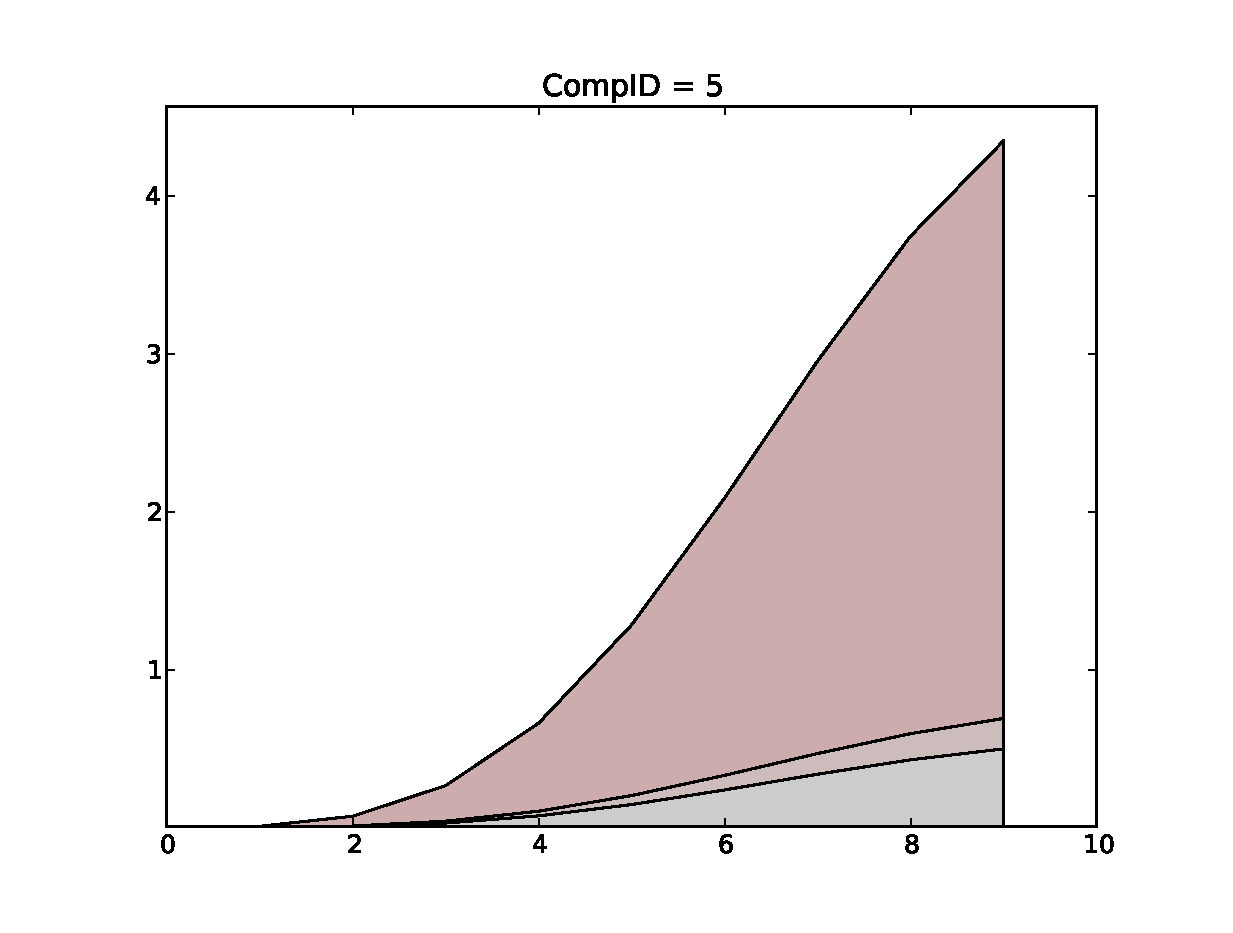
\includegraphics[width=0.5\textwidth]{cyder/images/deg_comp5.eps}
      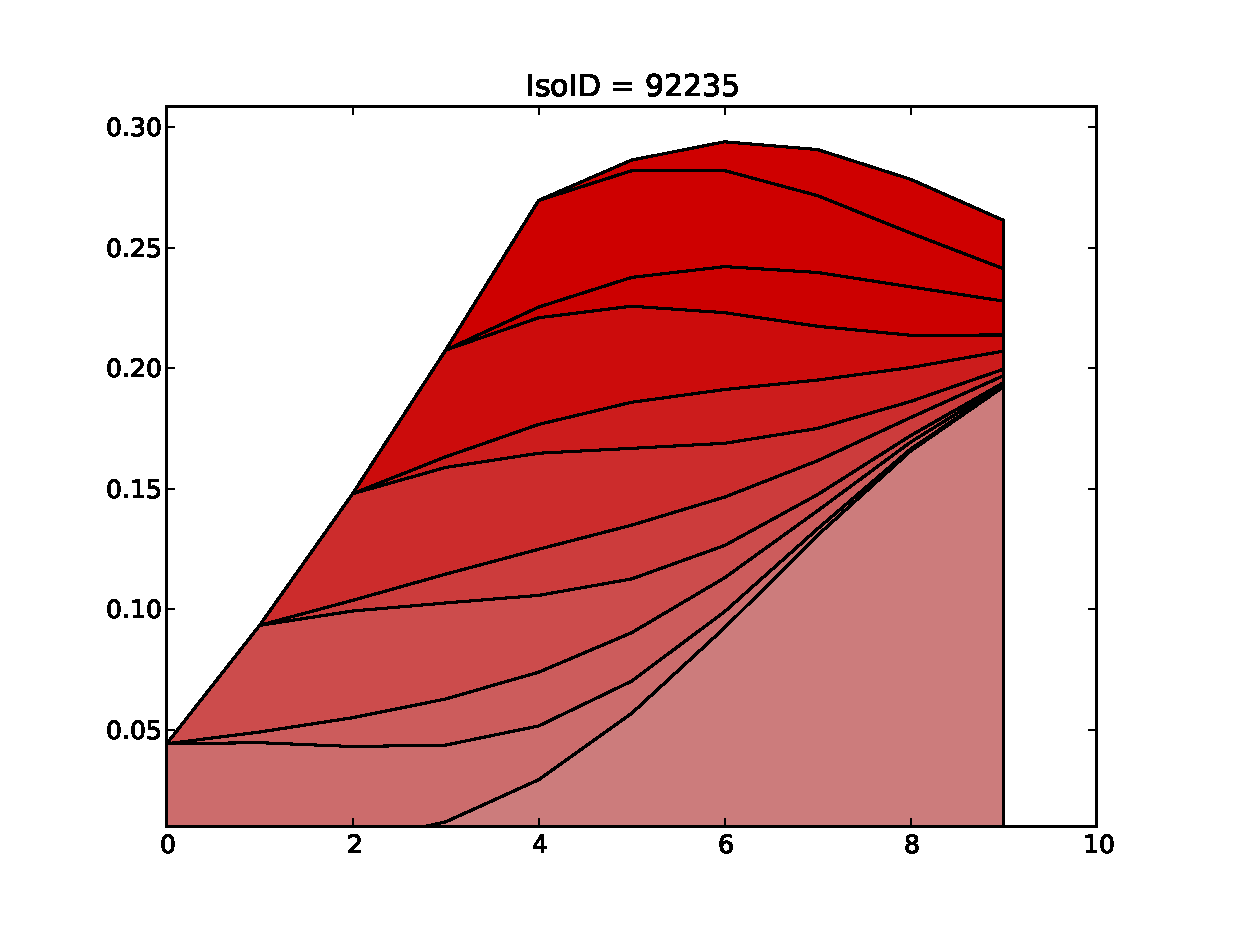
\includegraphics[width=0.5\textwidth]{cyder/images/deg.eps}
    \end{center}
  \end{figure}
\end{frame}

\begin{frame}
  \frametitle{Mixed Cell Base Case I}
  Base Case I : With no sorption or solubility constraints, it should behave very similarly to 
  the degradation cases, and indeed it does. If the solubility and sorption 
  constraints are added, their effect is expected to be miniscule over the 
  timeline of the simulation, 10 timesteps. Indeed it is. 

  \begin{figure}[htbp!]
    \begin{center}
     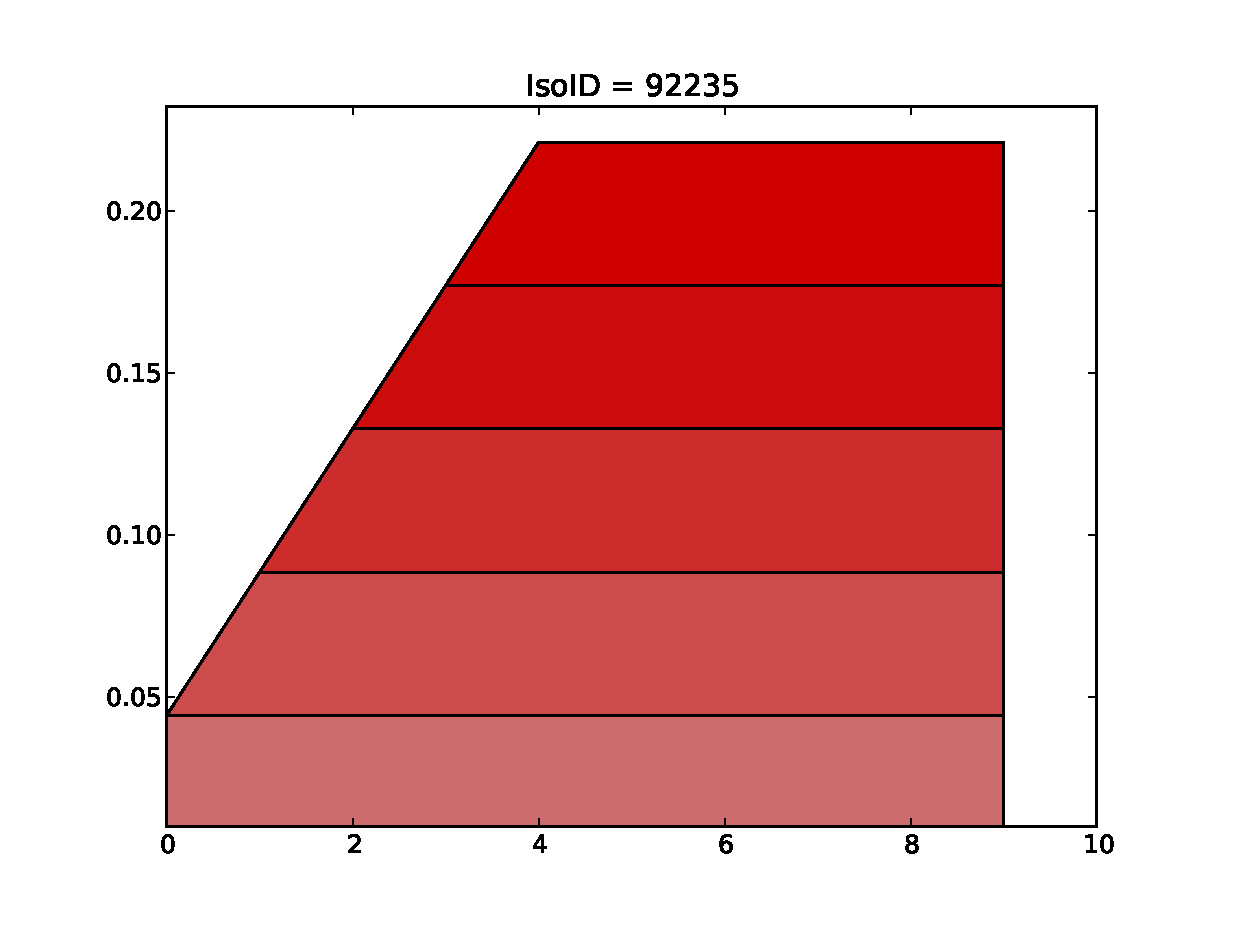
\includegraphics[width=0.5\textwidth]{cyder/images/mixed_0deg.eps}
     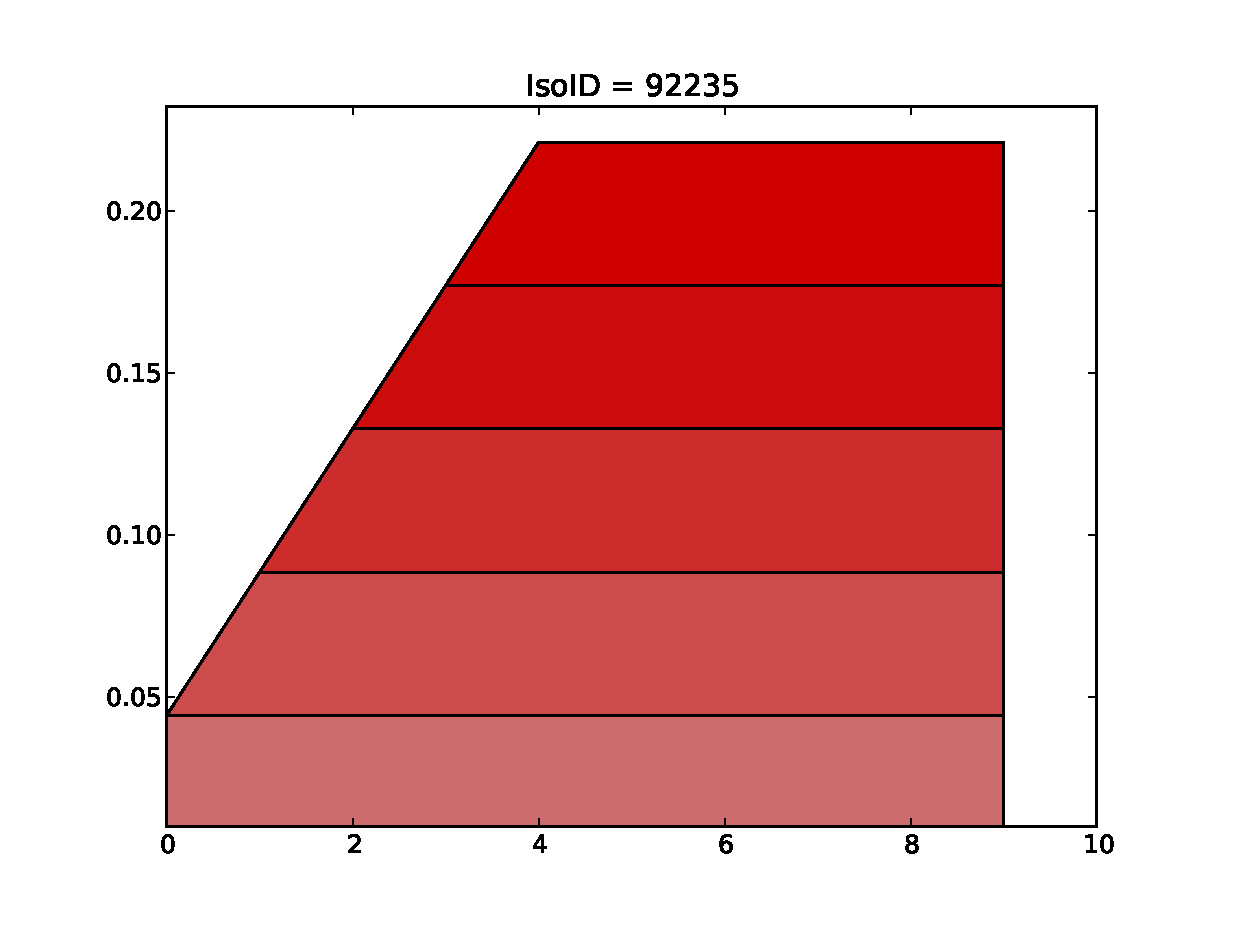
\includegraphics[width=0.5\textwidth]{cyder/images/0deg.eps}
     \caption{Left: Mixed Cell Nuclide Model, 0 degradation waste form, Solubility 
     limitation and Sorption activated. Right: Degradation Rate Nuclide Model, 0 degradation waste form, no 
     Solubility or Sorption}
    \end{center}
  \end{figure}
\end{frame}

\begin{frame}
  \frametitle{Mixed Cell Base Case II}
  Base Case II : With degradation of the waste form, the mixed cell model also 
  behaves similarly to the degradation rate model. 

  \begin{figure}[htbp!]
    \begin{center}
     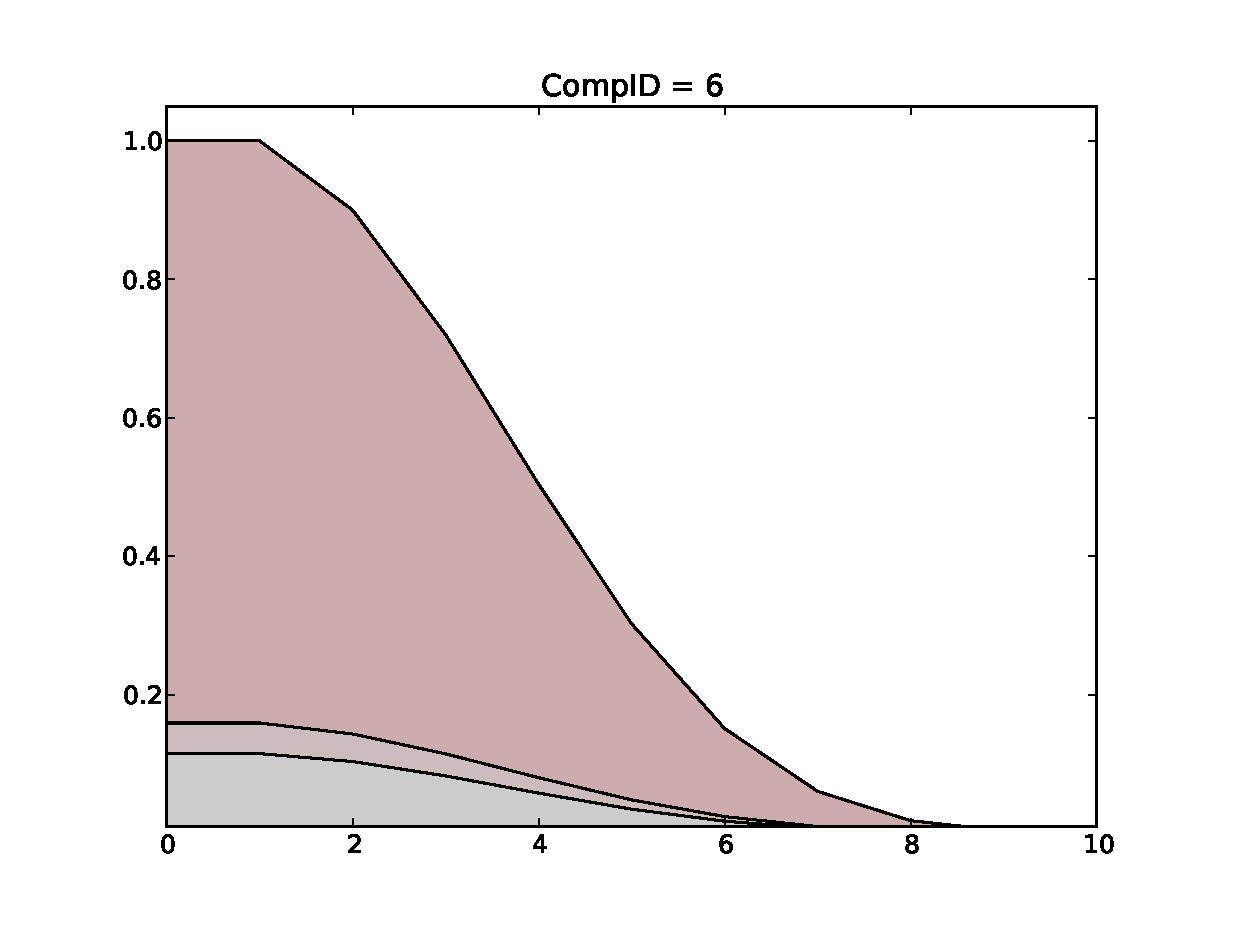
\includegraphics[width=0.5\textwidth]{cyder/images/mixed_comp6.eps}
     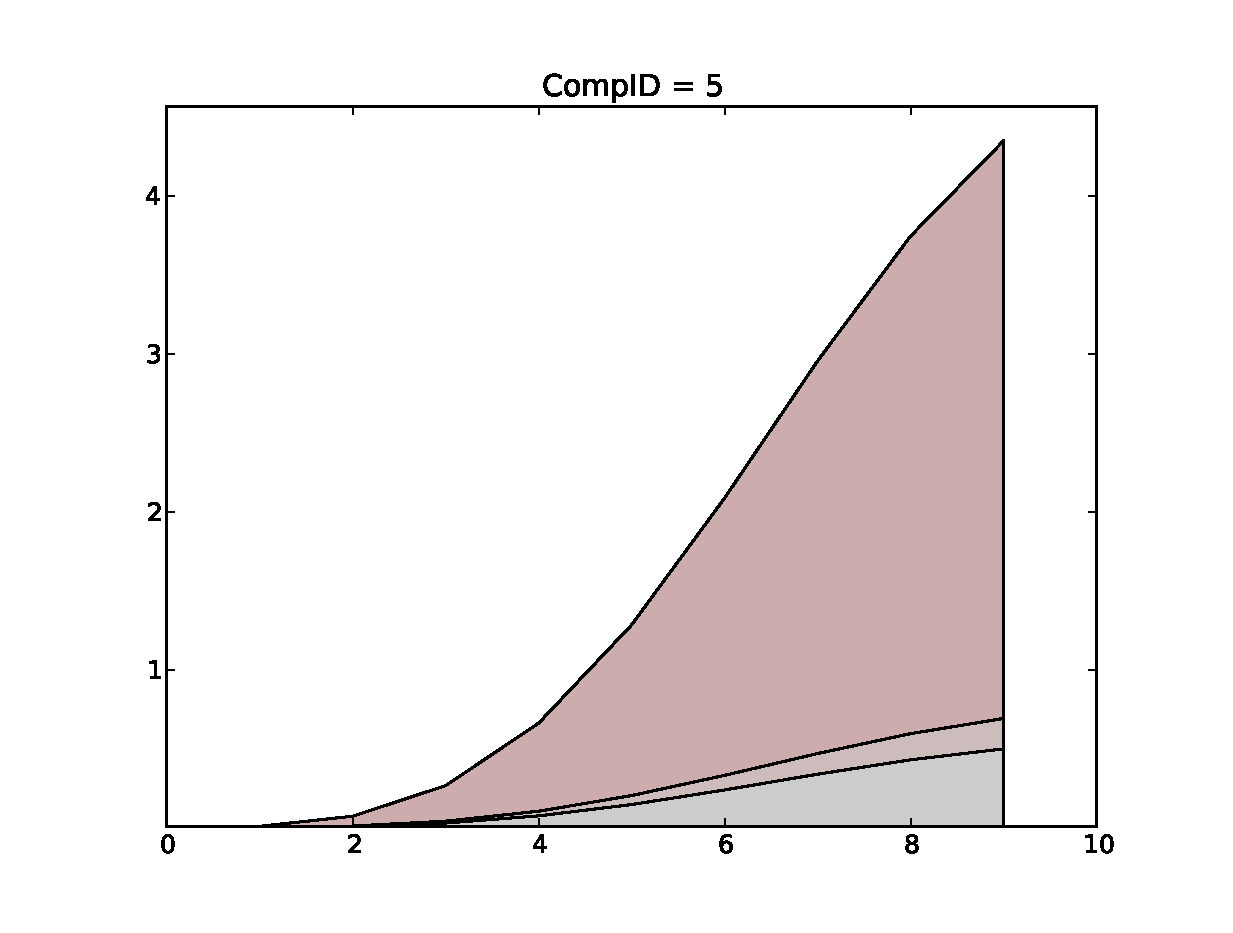
\includegraphics[width=0.5\textwidth]{cyder/images/mixed_comp5.eps}
    \end{center}
  \end{figure}
\end{frame}


